\documentclass[a4paper,10pt]{scrartcl}
\renewcommand{\familydefault}{\sfdefault}
\usepackage{helvet}
\usepackage{geometry}
\geometry{a4paper, top=25mm, left=30mm, right=25mm, bottom=30mm,
headsep=10mm, footskip=12mm}

\usepackage[T1]{fontenc}
\usepackage[utf8]{inputenc}
\usepackage[onehalfspacing]{setspace}
\usepackage{pdfpages}
\usepackage{bigfoot}
\usepackage{ulem}     % zum durchstreichen
\normalem
\usepackage{fancyvrb}
%\usepackage[usenames,dvipsnames]{xcolor}

\usepackage{blindtext}
\usepackage{cprotect}
\usepackage{hologo}   % for BibTex Logo

\usepackage[english,main=ngerman]{babel}
\usepackage{multibib}
\newcites{books,incoll,journals,web}{Beispiel: Monographie,%
Beispiel: Sammelb\"ande,%
Beispiel: Zeitschriftenartikel,%
Beispiel: Webseiten}
\usepackage{natbib}
\setlength{\bibhang}{0em}     % Quellen ohne hängenden Einzug im Literatur-
			      % verzeichnis

\renewcommand{\cite}{\citep}  %
\bibliographystyle{humanmutationTUD}     % angepasste Stildatei
\addto\captionsngerman{\renewcommand{\refname}{Literaturverzeichnis}}

\usepackage[%
   breaklinks            % Links ueberstehen Zeilenumbruch
  ,colorlinks            % Links erhalten Farben statt Kaesten
                         % keine bunten Farben verwendet
  ,citecolor=blue        % Farbe fuer Zitate
  ,linkcolor=blue        % beeinflusst Inhaltsverzeichnis und Seitenzahlen
  ,urlcolor=blue         % Farbe fuer URLs
  ]
  {hyperref}             % PDF automatisch mit Links versehen und weitere
                         % Hypertext-Funktionalitaet ermoeglichen
\def\UrlFont{\sffamily}  % URLs in Sans Serif


%opening
\title{Anpassungen des Stils \emph{Human Mutation} an die
Richtlinien der Medizinischen Fakultät Carl Gustav Carus, TU Dresden}
\subtitle{v0.3 vom 16.~Mai 2017}
\author{Daniel Kotik\\
\large\url{https://github.com/DanielKotik/BibTeX-Medicine-TU-Dresden}\\
\large\url{kotik@physics.org}}
\date{}

\begin{document}
\setlength{\parindent}{0em}
\maketitle

\begin{abstract}
Zur Umsetzung der Zitations- und Bibliographievorgaben für Dissertationen an
der Medizinischen Fakultät der TU~Dresden unter Verwendung von \LaTeX\ mit
\hologo{BibTeX} wird die Bibliographie Stil Datei
\verb|humanmutationTUD.bst| bereitgestellt. Die vorliegende Dokumentation gibt
Erläuterungen und allgemeine Hinweise zur korrekten Verwendung dieser Stil
Datei.
\end{abstract}

\section{Allgemeine Hinweise}
Die Zitations- und Bibliographievorgaben \cite{ZitiervorgabenCGC} der
Medizinischen Fakultät Carl Custav
Carus, TU~Dresden sind an den Stil der Zeitschrift Human
Mutation\footnote{\url{%
http://onlinelibrary.wiley.com/journal/10.1002/(ISSN)1098-1004}} angelehnt.
Zur Erfüllung der Vorgaben der Richtlinie muss der Stil unter anderem zusätzlich
an die der jeweiligen Referenz zugrunde liegenden Sprache angepasst werden um
sprachabhängige Abkürzungen in der Bibliographie zu ermöglichen (zum Beispiel
"`Hrsg"' oder "`ed"' bzw.\ "`eds"').
Hierfür wird eine optionale Feldvariable \verb|language={...}|
bereitgestellt, welche zusätzlich die korrekte sprachabhängige Silbentrennung
des Titels der Referenz gewährleistet\footnote{Hierfür wird das Paket
\verb|babel| genutzt.}. Fehlt die Angabe dieser Feldvariablen oder bleibt sie
leer, so wird standardmä{\ss}ig Englisch als Sprache für die jeweilige Referenz
angenommen.

Die Stildatei \verb|humanmutationTUD.bst| unterstützt folgende Literaturtypen:
\verb|article|, \verb|book|, \verb|booklet|, \verb|inbook|,
\verb|incollection|, \verb|inproceedings|(=\verb|conference|), \verb|manual|,
\verb|mastersthesis|, \verb|misc|, \verb|phdthesis|, \verb|proceedings|,
\verb|techreport|, \verb|unpublished|, \verb|webpage|.

%TODO: Angaben, welche Typen besonders durch den Stil beeinflusst werden (book,
%inpriceedings, webiste, unpublished). --> neuer Typ 'website'

Im Literaturverzeichnis des vorliegenden
Dokuments findet der hier
dargelegte Bibliographiestil bereits Anwendung. \\\\
Es sein darauf verwiesen, dass die unter \cite{humanmutationSchneider}
verfügbaren Stil- und Paketdateien \verb|humanmutation.bst| und
\verb|humanmutation.sty| veraltet sind und auch nicht den zusätzlichen Vorgaben
nach \cite{ZitiervorgabenCGC} entsprechen.

\section{Integration in \LaTeX}
In der Präambel sind folgende Pakete einzubinden und Kommandos (optional) zu
definieren:
\begin{singlespace}
\begin{Verbatim}[frame=single]
\usepackage[english,main=ngerman]{babel}  % Laden der Spachpakete mit Deutsch
                                          % als Standardsprache im Hauptdokument

\usepackage{natbib}  % notwendig zur Umsetzung des Zitiertils (Autor[en], Jahr) im
                     % Fliesstext

\setlength{\bibhang}{0em}  % Quellen ohne hängenden Einzug im Literaturverzeichnis

\renewcommand{\cite}{\citep}  % optional, falls nicht mit dem durch natbib
                              % bereitsgestellten \citep{}, sondern mit \cite{}
                              % gearbeitet werden möchte

\bibliographystyle{humanmutationTUD}  % angepasste Bibliographiestildatei ohne
                                      % Endung '.bst' angeben
\usepackage[%
  breaklinks,            % Links ueberstehen Zeilenumbruch
  colorlinks,            % Links erhalten Farben statt Kaesten
  citecolor=blue,        % Farbe fuer Zitate
  linkcolor=blue,        % beeinflusst Inhaltsverzeichnis und Seitenzahlen
  urlcolor=blue          % Farbe fuer URLs
]{hyperref}              % PDF automatisch mit Links versehen und weitere
                         % Hypertext-Funktionalitaet ermoeglichen
\def\UrlFont{\sffamily}  % verhindert URLs in Schreibmaschinenschrift
\end{Verbatim}
\end{singlespace}

Die Stildatei \verb|humanmutationTUD.bst| muss sich im gleichen Ordner wie
das Hauptdokument (bspw.\ \verb|dissertation.tex|) befinden. Zur Erstellung
des finalen PDF Dokuments sind üblicherweise drei \hologo{pdfLaTeX} Durchläufe
und ein \hologo{BibTeX} Durchlauf erforderlich, und zwar in folgender
Reihenfolge:\\
\begin{center}
 \begin{minipage}{0.7\textwidth}
  \verb|pdflatex dissertation.tex|\\
  \verb|bibtex dissertation.aux|\\
  \verb|pdflatex dissertation.tex|\\
  \verb|pdflatex dissertation.tex|
 \end{minipage}
\end{center}


%TODO: Erklären wo die bst Datei liegen muss und Ablauf pdflatex --> bibtex etc.

\section{Möglichkeiten zum Zitieren}
Im Folgenden wird gezeigt wie verschiedene Literaturtypen (Bücher,
Sammelbände, Artikel und Webseiten) korrekt unter Verwendung der Stildatei
\verb|humanmutationTUD.bst| zitiert werden.
\subsection{Zitieren von Büchern und Monographien}
Da es sich bei \citebooks{Schuhmacher2005} um ein deutsches Werk handelt, ist
die Angabe von \verb|language={ngerman}| im entsprechenden Eintrag der
\verb|.bib|~Datei erforderlich.
%TODO: Wird für ein englisches Buch der Titel verändert (Gross/Kleinschreibung)?

\cprotect{\noindent\makebox[1.0\textwidth][c]}{%
\small
\begin{minipage}[t]{1.2\textwidth}
    \begin{minipage}[t][5cm][c]{0.527\textwidth}
      %\hrulefill
      \begin{singlespace}
      \begin{Verbatim}[frame=single,commandchars=\\\(\)]
@book{Schuhmacher2005,
  title     = {Prometheus: Allgemeine Anatomie und
               Bewegungssystem -- LernAtlas der Anatomie},
  author    = {Schuhmacher, U and Schulte, E and
               Schünke, M},
  year      = {2005},
  (\color(red)language  = {ngerman},)
  edition   = {3},
  publisher = {Thieme},
  address   = {Stuttgart}
}
     \end{Verbatim}
     \end{singlespace}
     %\hrulefill
    \end{minipage}
    \hfill
    \begin{minipage}[t][5cm][c]{0.45\textwidth}
      %\hrulefill
      \bibliographybooks{example}
      \bibliographystylebooks{humanmutationTUD}
      %\hrulefill
    \end{minipage}
\end{minipage}
}

\subsection{Zitieren von Arbeiten in Sammelbänden}
Anhand von~\citeincoll{incollection_a} und~\citeincoll{incollection_b} werden
die sprachbedingten Unterschiede in der Bibliographie beim Zitieren von
Sammelb\"anden verdeutlicht. Auch hier gilt, dass die Angabe von
\verb|language={ngerman}| im ersten Eintrag notwendig, die Angabe von
\verb|language={english}| im zweiten Eintrag hingegen nicht zwingend
erforderlich ist (Englisch ist Standard). Das Feld \verb|note| ist generell
optional. Die Zeichenkette im Feld
\verb|booktitle| wird unverändert in der Bibliographie
wiedergegeben (d.h.\ keine sprachbedingte Veränderung der Gro{\ss}- und
Kleinschreibung wie bei
\verb|title|, aber korrekte Silbentrennung entsprechend der Sprache im
\verb|language| Feld).

\cprotect{\noindent\makebox[1.0\textwidth][c]}{%
\small
\begin{minipage}[t]{1.15\textwidth}
    \begin{minipage}[t][13cm][c]{0.522\textwidth}
      %\hrulefill
      \begin{singlespace}
      \begin{Verbatim}[frame=single,commandchars=\\\(\)]
@incollection{incollection_a,
  author      = {Dirac, Paul},
  title       = {Titel der fiktionalen Arbeit},
  booktitle   = {Titel des fiktionalen Buches},
  publisher   = {Name des Verlegers},
  year        = 1950,
  editor      = {Einstein, Albert and Pauli, Wolfgang},
  volume      = 4,
  series      = 5,
  chapter     = 8,
  pages       = {201-213},
  address     = {Verlagsanschrift},
  edition     = {3},
  (\color(red)language    = {ngerman},)
  note        = {Ein optionaler Hinweis}
}

@incollection{incollection_b,
  author      = {Dirac, Paul},
  title       = {The Title of the fictional Work},
  booktitle   = {The Title of the fictional Book},
  publisher   = {The name of the publisher},
  year        = 1950,
  editor      = {Einstein, Albert and Pauli, Wolfgang},
  volume      = 4,
  series      = 5,
  chapter     = 8,
  pages       = {201-213},
  address     = {The address of the publisher},
  edition     = {3},
  (\color(red)language    = {english},)
  note        = {An optional note}
}
     \end{Verbatim}
     \end{singlespace}
     %\hrulefill
    \end{minipage}
    \hfill
    \begin{minipage}[t][13cm][c]{0.45\textwidth}
      %\hrulefill
      \bibliographyincoll{example}
      \bibliographystyleincoll{humanmutationTUD}
      %\hrulefill
    \end{minipage}
\end{minipage}
}

\subsection{Zitieren von (unver\"offentlichten) Artikeln}
Anhand von~\citejournals{vonSchulthess2010} wird das Zitieren eines
bereits veröffentlichten Artikels und von~\citejournals{Cronin2017} eines noch
unveröffentlichten Artikels
verdeutlicht. Für den Literaturtyp \verb|unpublished| wird ein
zusätzliches Feld \verb|doi={...}| zur Angabe des DOI (\textbf{D}igital
\textbf{O}bject \textbf{I}dentifier) bereitgestellt\footnote{Das Vorhandensein
des Feldes \verb|doi={...}| bleibt für alle anderen Literaturtypen ohne
Wirkung.}. Das optionale \verb|language| Feld beeinflusst den Hinweis auf einen
sich im Druck befindlichen, d.h.\ bisher unveröffentlichten Artikel ("`[im
Druck]"' für \verb|ngerman| bzw.\ "`[in press]"' für die englische und alle
anderen Sprachen). Der DOI wird automatisch dem DOI Resolver
\url{https://dx.doi.org/} übergeben und verlinkt. Ein eventuell vorhandenes
Feld \verb|month| bleibt ohne Wirkung.

% \footnote{Unveröffentlichte Artikel, welche auf PubMed gelistet
% sind, können mit \url{ http://www.bioinformatics.org/texmed/} ansatzweise in
% Bibtex umgewandelt werden.}


\cprotect{\noindent\makebox[1.0\textwidth][c]}{%
\small
\begin{minipage}[t]{1.25\textwidth}
    \begin{minipage}[t][9cm][c]{0.53\textwidth}
      %\hrulefill
      \begin{singlespace}
      \begin{Verbatim}[frame=single,commandchars=\\(\)]
@unpublished{Cronin2017,
   author  = {Cronin, O. and Keohane, D. M. and Molloy, M. G.
              and Shanahan, F.},
   title   = {The effect of exercise interventions on
             inflammatory biomarkers in healthy, physically
             inactive subjects: a systematic review},
   (\color(red)doi     = {10.1093/qjmed/hcx091},)
   journal = {QJM},
   year    = {2017},
   month   = {May}
}

@article{vonSchulthess2010,
   author  = {von Schulthess, G. K. and Burger, C.},
   title   = {Integrating imaging modalities: what
              makes sense from a workflow perspective?},
   journal = {Eur J Nucl Med Mol Imaging},
   volume  = {37},
   number  = {5},
   pages   = {980-990},
   month   = 10,
   year    = {2010}
}
     \end{Verbatim}
     \end{singlespace}
     %\hrulefill
    \end{minipage}
    \hfill
    \begin{minipage}[t][9cm][c]{0.45\textwidth}
      %\hrulefill
      \bibliographyjournals{example}
      \bibliographystylejournals{humanmutationTUD}
      %\hrulefill
    \end{minipage}
\end{minipage}
}

\subsection{Zitieren von Webseiten}
Zum Zitieren von Webseiten wird durch die Bibliographiestildatei
der Literaturtyp \verb|webpage| zur Verfügung gestellt. Webseiten können
damit auf zweierlei Weise zitiert werden. Beide Varianten seien hier
beispielhaft an~\citeweb{humanmutationSchneider} sowie die diesem Dokument
zugrunde liegenden Zitiervorgaben
\citeweb{ZitiervorgabenCGC} erläutert. Beide Varianten unterscheiden sich
lediglich in der Angabe des~URL: Für äußerst lange bzw.\ unhandliche
URLs\footnote{Zum
Beispiel der originale URL von \cite{ZitiervorgabenCGC}: \url{
https://tu-dresden.de/med/mf/ressourcen/dateien/postgraduales/promotionen/zitier
richtinien_fuer_die_dissertation_formblatt9.0?lang=de}.} empfiehlt es sich
einen kurzen Alias (short URL)\footnote{Beispielhaft genannt seien hier die
Dienste \url{https://goo.gl/} und \url{https://bitly.com/}.} mittels
\verb|shorturl={...}| anzugeben. Verliert der Link später seine Gültigkeit oder
ändert sich die Adresse, wird durch die Angabe des Hostnames \verb|host={...}|
(und der ersten Teilpfade) zusätzlich kenntlich gemacht, wo die Datei
ursprünglich im WWW aufzufinden war. Dadurch kann auch später die Datei oder
Webseite, sofern noch vorhanden, möglicherweise wiedergefunden werden, selbst
wenn sich der ursprüngliche URL geändert hat. Für kurze URLs kann dieser direkt
dem Feld \verb|url={...}| übergeben werden.

Für eine korrekte Silbentrennung  des Titels sollte bei einer deutschsprachigen
Webseite zudem zusätzlich
\verb|language={ngerman}| mit eingetragen werden. Dem Feld
\verb|lastrevised={...}|
kann optional das Datum der letzten Änderung der Webseite übergeben werden
(date of last revision). Das Datum des Webseitenaufrufs hingegen ist zwingend
erforderlich und muss als Wert dem Feld
\verb|lastchecked={...}| übergeben werden (falls nicht, wird eine
Warnung beim Kompilieren mit \hologo{BibTeX} ausgegeben).

\cprotect{\noindent\makebox[1.0\textwidth][c]}{%
\small
\begin{minipage}[t]{1.2\textwidth}
    \begin{minipage}[t][9cm][c]{0.527\textwidth}
      %\hrulefill
      \begin{singlespace}
      \begin{Verbatim}[frame=single,commandchars=&\(\)]
@webpage{ZitiervorgabenCGC,
  author   = {Bilz, Alexander},
  year     = 2013,
  title    = {Zitierrichtlinien f{\"u}r Dissertationen an
              der Medizinischen Fakultät der TU Dresden},
  language = {ngerman},
  url      = {},
  (&color(red)shorturl = {https://goo.gl/DbLwTW},)
  (&color(red)host     = {https://tu-dresden.de/med/mf},)
  (&color(red)lastchecked = {27.04.2017},)
  (&color(red)lastrevised = {})
}

@webpage{humanmutationSchneider,
  author = {Schneider, Thomas},
  year   = 1998,
  title  = {\hologo{BibTeX} `humanmutation' bibliography
            style},
  url    = {https://schneider.ncifcrf.gov/latex.html},
  (&color(red)lastchecked = {05.05.2017},)
  (&color(red)lastrevised = {27.05.2016})
}
     \end{Verbatim}
     \end{singlespace}
     %\hrulefill
    \end{minipage}
    \hfill
    \begin{minipage}[t][9cm][c]{0.45\textwidth}
      %\hrulefill
      \bibliographyweb{example}
      \bibliographystyleweb{humanmutationTUD}
      %\hrulefill
    \end{minipage}
\end{minipage}
}

\subsection{Fallstricke}
Hier zitieren wir den Artikel~\cite{Teras2016_FALSCH} und noch einmal in
verbesserter Form~\cite{Teras2016_RICHTIG}. Beide Zitate referenzieren
tats\"achlich die gleiche Quelle, nur das beim zweiten Zitat der
Titel auch \emph{korrekt} in der Bibliographie angezeigt wird. Der
marginale Unterschied des entsprechenden Eintrages
in der \verb|.bib|~Datei besteht im Folgendem:\\\\
\emph{falsch}
\begin{Verbatim}
title = {2016 US lymphoid malignancy statistics by World Health Organization
         subtypes},
\end{Verbatim}
\emph{richtig}
\begin{Verbatim}[commandchars=\\\(\)]
title = {2016 (\color(red){)US(\color(red)}) lymphoid malignancy statistics by World Health Organization
         subtypes},
\end{Verbatim}
Durch die zusätzlichen geschweiften Klammern um \texttt{US} wird erreicht, dass der Titel
auch korrekt wiedergegeben wird. Andernfalls wird bei englischsprachigen
Referenzen durch \hologo{BibTeX} die gesamte Zeichenkette zwischen den
\"au{\ss}ersten Klammern \texttt{\{\ldots \}} in Kleinschrift gesetzt und
\emph{nur der erste} Buchstabe gro{\ss} gesetzt (gewünschtes Verhalten). Es empfiehlt sich daher händisch in
der
\verb|.bib|~Datei alle Titel Einträge sorgfältig zu überprüfen, auch um
gegebenenfalls überflüssige Klammern \emph{zu entfernen}\footnote{Abhängig vom
Tool mit welchem Referenzen gesammelt und später in \hologo{BibTeX}-Einträge
umgewandelt werden (Zotero, Jabref, Endnote, Google Scholar etc.), wird
eventuell für alle im Titel vorkommenden Wörter
Gro{\ss}- und Kleinschreibung forciert; in obigem Beispiel bspw.\ \verb|{W}orld {H}ealth {O}rganization|.},
so dass ein einheitliches Bild im Literaturverzeichnis gewährleistet ist.

\section{Technisches}
Die Datei \verb|human.dbj| kann in einem Texteditor manuell angepasst
werden\footnote{%
\url{https://ftp.fau.de/ctan/macros/latex/contrib/custom-bib/merlin.pdf}} um
gegebenenfalls Änderungen am Stil der Referenzen im Literaturverzeichnis
vorzunehmen.
%TODO: Zusammenhang mit makebst erläutern


\section{To Do}
\begin{itemize}
 \item Fertigstellung der Dokumentation
 \item \sout{Hinweis auf inoffiziellen Status, changelog und Version in Stil
Datei
einfügen}
 \item Auflage: Angabe nur ab 2.~Auflage aufwärts
 \item korrekte Angabe der Auflage, d.h.\ "`2.~Aufl."', "`2.~erw. Aufl."', "`2nd
ed."'
 \item \sout{Erstellen eines eigenen Eintrags für Webseiten (zum Beispiel}
\verb|@webpage|\sout{), mit Feldern für \emph{URL} (alternativ \emph{short URL}
und
\emph{hostname}) sowie Felder für \emph{Aufruf am} und
\emph{Aktualisiert am} (v0.3). Es gilt zu
beachten,
dass die URL nicht im typewriter Font angegeben werden soll. Eventuell muss das
Paket hyperref bzw. url sinnvollerweise geladen werden.}
\item korrekter Umgang mit Journalabkürzungen
\item \sout{Hinweis (in press) bzw.\ (im Druck) mit DOI f\"ur im Druck
befindliche und
vorab elektronisch ver\"offentlichte Artikel (v0.2)}
\end{itemize}


\newpage
\label{sec:Literaturverzeichnis}
\bibliography{example}
\nocite{*}

%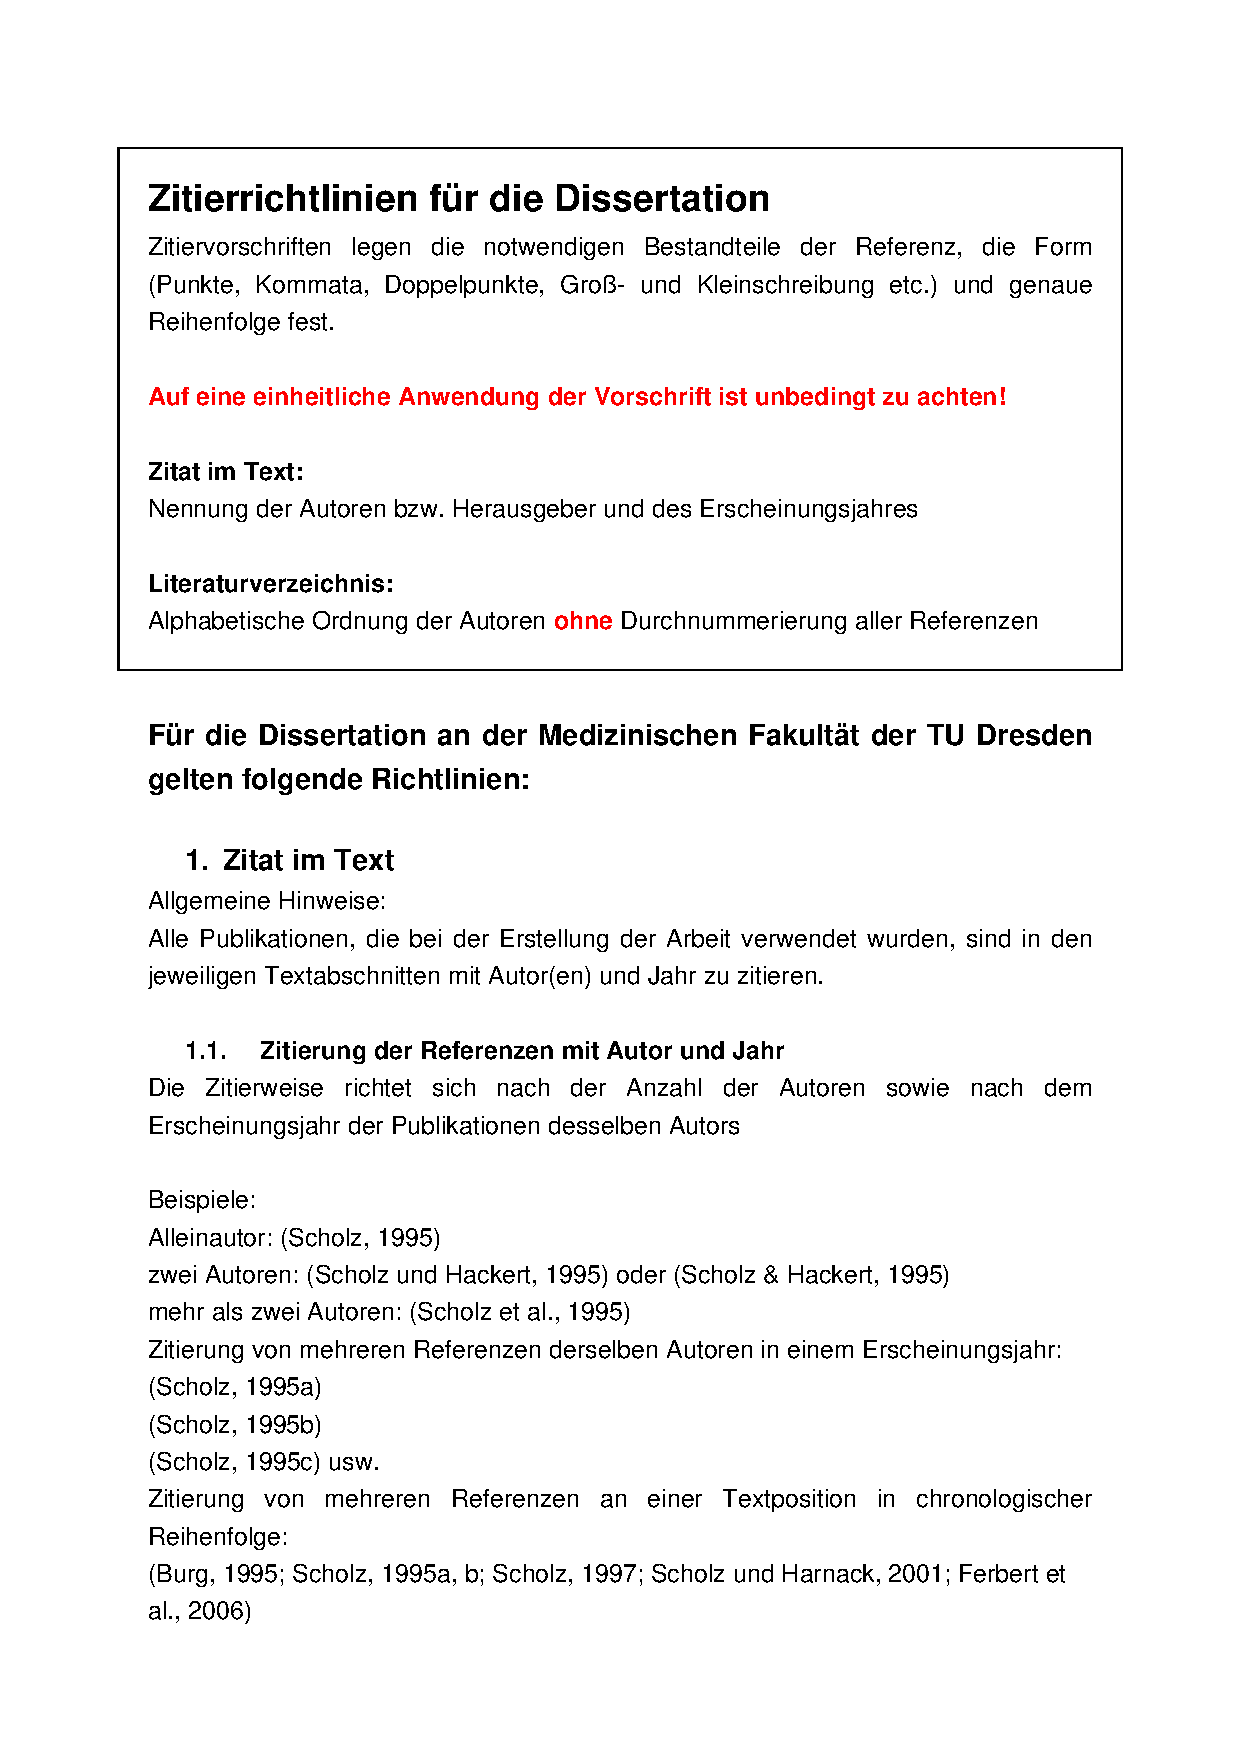
\includepdf[pages={-}]{zitierrichtinien_fuer_die_dissertation_formblatt9.pdf}

\end{document}
